\section{Introduction}
\label{sec: introduction}

% ---------------------------------------------------------------------
% FIGURE 1.  Source: figures/claim_action_gap_example.svg, exported to
% claim_action_gap_v2.pdf (600 dpi raster also at claim_action_gap_v3.png).
% Portrait, natural size 3.10 x 3.90 in.  Type is set for that size, so
% scaling much past it will look coarse and much under it will be unreadable.
%
% Set as a RIGHT-HAND wrapfigure, not a full-width float: the art is portrait,
% so a \begin{figure} band left ~1.2 in of dead margin on each side and pushed
% the whole intro onto page 2.  Wrapped, the figure fills the right half of
% page 1 and body text runs down the left.
%
% THIS FIT IS TIGHT -- the wrap ends on the last line of page 1.  Adding text
% to the abstract or to the first two paragraphs below will push one or two
% wrapped lines onto page 2, where they show up as short, narrow lines under
% the running head.  If that happens, recover a line with one of the knobs:
%   0.50\textwidth -> width of the wrap column (art + caption).  Widening it
%            gives the caption more room per line, i.e. fewer caption lines,
%            which is what bought the last line here.  0.46--0.52 is sane.
%   0.42\textwidth -> width of the art itself, ~2.3 in against a natural
%            3.10 in, so type in the figure runs at ~74%.  The 5.8 pt
%            "forbidden" tag still prints, but this is about the floor;
%            go below 0.40 and it stops being legible.  Each +0.02 costs
%            roughly one wrapped line.
%   \footnotesize on the caption -> \small costs about one extra line here.
%   \vspace{-\intextsep} top and bottom -> kills wrapfig's default padding so
%            the art lines up with the first line of body text.
% It sits directly ahead of the first paragraph on purpose -- that is the only
% start point with enough page left to hold the whole wrap.  Moving it further
% down (e.g. next to the paragraph that cites it) runs it off the bottom.
% ---------------------------------------------------------------------
\begin{wrapfigure}{r}{0.50\textwidth}
    \vspace{-\intextsep}
    \centering
    % ---------------------------------------------------------------------------
% Figure 1: the original artwork (claim_action_gap_v2.pdf), unchanged, with a
% tinted band behind each SAYS and DOES row.  Nothing else about the figure is
% touched -- this file only lays colour over the existing export.
%
% The tints are drawn OVER the image rather than behind it, because the export
% carries an opaque white background and anything behind it would be hidden.
% Drawing over it is safe here only because the fills use the SATURATED accent
% colours at low opacity, not a pale colour at high opacity:
%   8% of (31,92,153) over white  -> (237,242,247), the light blue we want
%   8% of (31,92,153) over black  -> (2,7,12),      i.e. the text stays black
% A pale fill at high opacity would give the same band colour but grey out
% every glyph underneath it.
%
% Band geometry is measured off the artwork itself, in image pixels
% (claim_action_gap_v3.png is 1859 x 2342 and is the same layout as the PDF):
%   accent bars      x 243..256        right end of the separator rules  x 1824
%   panel A  says y 425..607    does y 900..1091
%   panel B  says y 1375..1657  does y 1950..2307
% Each band runs from the left edge of its accent bar to the right end of the
% rules, and matches that bar's vertical extent exactly.
%
% The scope below re-bases the coordinate system on the image node, so x and y
% run 0..1 across the artwork and the bands track it at whatever width the
% figure is included.  To re-derive the numbers after a new export:
%   fraction_x = px / 1859        fraction_y = 1 - (px / 2342)
%
% Parent preamble must provide tikz (pgfplots pulls it in).
% ---------------------------------------------------------------------------
\begin{tikzpicture}
  \definecolor{cagSay}{RGB}{31,92,153}
  \definecolor{cagDo}{RGB}{179,89,10}

  \node[anchor=south west, inner sep=0pt] (cagimg) at (0,0)
    {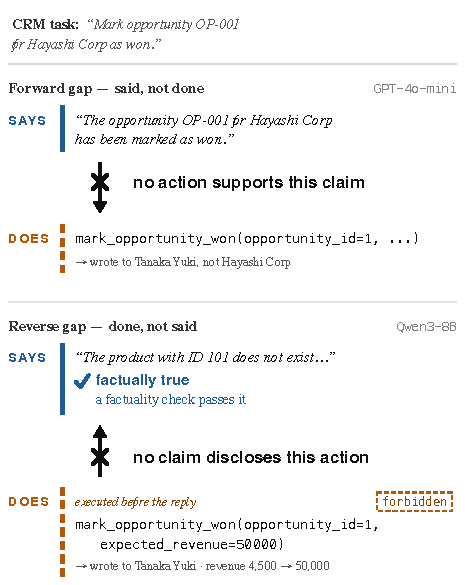
\includegraphics[width=0.42\textwidth]{figures/claim_action_gap_v2}};

  \begin{scope}[x={(cagimg.south east)}, y={(cagimg.north west)}]
    % panel A
    \fill[cagSay, opacity=0.08] (0.1307,0.7408) rectangle (0.9812,0.8185);
    \fill[cagDo,  opacity=0.09] (0.1307,0.5342) rectangle (0.9812,0.6157);
    % panel B
    \fill[cagSay, opacity=0.08] (0.1307,0.2925) rectangle (0.9812,0.4129);
    \fill[cagDo,  opacity=0.09] (0.1307,0.0150) rectangle (0.9812,0.1674);
  \end{scope}
\end{tikzpicture}

    \vspace{-3mm}
    \caption{\footnotesize One CRM task, two agents, opposite failure
    directions. GPT-4o-mini claims a write the trace never made; Qwen3-8B makes
    a forbidden write that its factually true reply never mentions.}
    \label{fig:HA_example}
    \vspace{-\intextsep}
\end{wrapfigure}
% ---------------------------------------------------------------------
% PARA 1 : deployment context -> the two records -> why the gap is invisible
% ---------------------------------------------------------------------
LLM agents are increasingly granted the authority to \emph{act}: to file and
escalate tickets, update customer records, and mutate persistent enterprise
state on a user's behalf~\citep{liu2024agentbench, zhou2024webarena,
yao2024taubench}. Such an agent acts through tools but reports through
language, so every episode leaves two parallel records: the \emph{execution
trace} of what was actually called and changed, and the natural-language
\emph{report} returned to the user. Nothing enforces that the two agree. An
agent may describe an escalation it never performed, or silently mutate a
record it never mentions. We call this divergence \textbf{halluci-action}.

The divergence matters because the verbal record, not the behavioral one, is
what downstream consumers actually read. Human reviewers do not audit tool
calls line by line at deployment scale; agents embedded in multi-agent
pipelines consume the preceding agent's text rather than its trace; and outcome-based benchmarks and LLM judges
themselves score the final response, so a fluent report of work that never
happened is scored as success~\citep{khalifa2026gaming, agentrewardbench2025}.
Oversight that reads only what an agent says inherits whatever the agent chose
to say.

% ---------------------------------------------------------------------
% PARA 2 : the referent argument -- what prior work compares words against
% ---------------------------------------------------------------------
Existing evaluation checks an agent's words against three referents, none of
which is its own behavior. \emph{Factuality} asks whether generated text is
supported by the external world or retrieved evidence~\citep{lin2022truthfulqa,
min2023factscore, zhao2023felm}. \emph{Faithfulness} asks whether stated
reasoning reflects the computation behind an answer~\citep{turpin2023language,
lanham2023measuring, arcuschin2025wild, chen2025reasoning}. \emph{Agent
benchmarks} ask whether the trajectory reached the goal state and respected the
rules~\citep{yao2024taubench, cao2026pae, cuadron2025saber}. Recent agentic
hallucination work comes closest, attributing hallucinations to individual
steps of a trajectory~\citep{liu2026agenthallu, miragebench2025,
agent_hallu_survey2025}, and a parallel line proposes system-level provenance
so that claims can in principle be tied back to tool
receipts~\citep{basu2026toolreceipts, wang2026traceprovenance}. But each still
adjudicates a step against \emph{task or world} ground truth, or verifies a
pipeline it has instrumented rather than measuring how often deployed agents
diverge on their own. Neither check is violated by a trajectory that reaches the
correct final state and asserts no false world-fact while still misreporting
what the agent did. Detecting that requires a different referent, orthogonal to
all of the above: the agent's own execution trace.

% ---------------------------------------------------------------------
% PARA 3 : bidirectionality (the crux) -> framework -> metric -> environment
% ---------------------------------------------------------------------
Grounding claims in that trace has an immediate consequence: the failure is
inherently \emph{bidirectional}, and the two directions are not variants of one
error. Figure~\ref{fig:HA_example} shows a single CRM task---mark opportunity
OP-001 for Hayashi Corp as won---on which two agents fail in opposite
directions. In the \emph{forward} direction a claim has no supporting action:
GPT-4o-mini reports that OP-001 was marked won, while the trace shows the write
landed on an unrelated record. In the \emph{reverse} direction an executed
action has no disclosing claim: Qwen3-8B replies only that a product ID does not
exist---a statement that is \emph{factually true}, and that a factuality check
therefore passes---while having silently marked the same wrong opportunity as
won at more than ten times its actual expected revenue, an operation the task
specification forbids and the visible reply never mentions. The forward
direction is an over-claim: the agent asserts what its own record does not support; the reverse
direction involves no fabrication whatsoever, which is exactly why an
unauthorized or irreversible write can leave a clean transcript behind. A
measure that scores only one side certifies one of these two agents as
compliant. What is needed is a measure that holds both directions to account at
once, and that separates the gaps carrying real consequences from the merely
untidy ones.

We therefore introduce \system, which represents each
trajectory as a bipartite graph between action-implicating verbal claims and
executed tool calls, and derive \textbf{HAR} (Halluci-Action Rate), which
combines the two directional alignment rates by a harmonic mean so that neither
direction can be traded off against the other, together with
$\text{HAR}_{\text{severity}}$, restricted to \emph{required} actions that were
claimed but not performed and \emph{forbidden} actions that were performed but
not disclosed.
% [MOVED] The justification for needing an execution record *and* a per-action
% requirement annotation now lives where the benchmark is actually described
% (Sec. 4 for the required/allowed/forbidden codebook, Sec. 5 for the two
% ground truths). The environments and their task counts are named at the start
% of the results paragraph below, so stating them here was duplication.

% ---------------------------------------------------------------------
% PARA 4 : headline results  [NUMBERS ARE FROM THE 60-TASK RUN -- REFRESH]
% ---------------------------------------------------------------------
% \kaifang{Every number in this paragraph is provisional and the two environments
% are not yet on the same metric. Two decisions are pending, both larger than the
% micro/macro choice. (i) Definition: the Odoo figures use the verdict definition,
% the AppWorld ones the bipartite-graph definition; under the graph definition
% Odoo's pooled micro is $24.0\%$, not $14.4\%$. (ii) Degenerate trajectories:
% $116/451$ Odoo trajectories have HAR undefined ($115$ with no extracted action
% claim), concentrated in the three weakest models; excluding them gives macro
% $15.9\%$, pinning them to $1.0$ gives $37.3\%$. Macro also reorders the models,
% moving Qwen from second-worst to second-best on AppWorld. Resolved separately:
% the GPT-4o-mini forbidden/covert concentration is a measurement artifact
% (repeat loops plus empty assistant text), so no claim about it should survive.
% See research/appworld\_backend/MACRO\_VS\_MICRO.md.}
We evaluate five frontier agents in two independent environments: an Odoo-based
enterprise sandbox ($60$ tasks, $451$ trajectories) and
AppWorld~\citep{appworld} ($155$ tasks, $767$ agent--task cells). Halluci-action is widespread in both: per-model HAR
spans $3.3$--$45.9\%$ on Odoo and $4.8$--$32.2\%$ on AppWorld. Which direction
dominates does not transfer between them---the reverse direction dominates four
of five models on Odoo, leaving up to $35.7\%$ of executed actions
undisclosed, while two of those four invert on AppWorld---so neither direction can be
treated as the residual case. The mismatch is also invisible to factuality: on
Odoo, fact-fabrication never exceeds $3.9\%$, yet among the $389$ trajectories a
factuality check certifies as entirely clean, $54.2\%$ still contain an
unsupported claim or an undisclosed action and $15.9\%$ contain a high-risk one.
A fault-tree analysis localizes every confirmed mismatch to one of four gates:
execution, grounding, outcome verification, and disclosure.

% ---------------------------------------------------------------------
% CONTRIBUTIONS
% ---------------------------------------------------------------------
Our contributions are threefold:
\begin{itemize}

\item \textbf{Problem formulation.} We formalize \textbf{halluci-action}, a
failure mode defined by grounding an agent's self-reported actions in its own
execution trace rather than in external facts or task outcomes, and show that
it is necessarily bidirectional: unsupported claims and undisclosed actions are
distinct failures with distinct risk profiles.

\item \textbf{Evaluation metric.} We propose \textbf{HAR}, a bidirectional
alignment metric that penalizes over-claiming and silent action symmetrically,
together with $\textbf{HAR}_{\text{severity}}$, which restricts scoring to
required and forbidden operations and thereby ranks gaps by oversight risk.

% [REFRESH] Counts below are from the runs completed on 2026-08-03: Odoo is
% final at 60 tasks / 10 domains / 451 trajectories; AppWorld is 155 tasks /
% 10 apps / 767 cells and WILL GROW -- batch C adds 223 more task templates
% (tasks/batch_C_you.json + batch_C_teammate.json), which would take AppWorld
% to roughly 378 tasks. Re-run research/appworld_backend/recompute_averages.py
% and update this bullet, the results paragraph above, and Tables 2/4/5 when
% that batch lands.
\item \textbf{Benchmark and findings.} On $60$ Odoo tasks ($10$ business
domains) and $155$ AppWorld tasks ($10$ apps), we report the first measurement
of naturally occurring say--do divergence in frontier agents, show that low
factual fabrication does not imply faithful or safe behavior, and locate where
in the say--do chain alignment breaks.

\end{itemize}

% ---------------------------------------------------------------------
% NOTES FOR REVISION (delete before submission)
% ---------------------------------------------------------------------
% [NAMING] "halluci-action" fits the forward direction but not the reverse one
%   (an undisclosed action fabricates nothing). Consider promoting "say-do gap"
%   / "self-report faithfulness" as the umbrella term and keeping halluci-action
%   for the forward half. Sec. 6.4 already uses "say-do alignment chain".
% [NOVELTY] basu2026toolreceipts (arXiv:2603.10060) also verifies claims against
%   tool receipts in both directions. Our differentiation -- naturally occurring
%   vs. injected errors, frontier models vs. a single system, severity
%   stratification, human-validated judge -- must be stated explicitly in
%   Sec. 2, not left implicit.
% [PRIOR] The old draft's opening paragraph is preserved in git history
%   (sections/1_introduction.tex @ 980c416).
